\documentclass[a4paper,11pt]{article}

\usepackage[french]{babel}
\usepackage[utf8]{inputenc}
\usepackage{lmodern}
\usepackage[T1]{fontenc}
\usepackage{graphicx}
\usepackage{fullpage}
\usepackage{lmodern}
\usepackage{caption}
\usepackage{subcaption}
\usepackage{placeins}
\usepackage[export]{adjustbox}
\usepackage{comment}
\usepackage{listings}
\usepackage{fancyhdr}
\usepackage{pdfpages}

\usepackage{url}
\usepackage{xcolor}
\newcommand{\cb}[1]{\textcolor{magenta}{#1}}

\usepackage{tikz}
\usetikzlibrary{shapes}
\usepackage{graphicx}

\usepackage{hyperref}
\hypersetup{
    colorlinks=true,
    linkcolor=blue,
    filecolor=magenta,      
    urlcolor=red,
    pdftitle={PDP IA Suggestion Musical},
    pdfpagemode=FullScreen,
}

\definecolor{codegreen}{rgb}{0,0.6,0}
\definecolor{codegray}{rgb}{0.5,0.5,0.5}
\definecolor{codepurple}{rgb}{0.58,0,0.82}
\definecolor{backcolour}{rgb}{0.95,0.95,0.92}

\lstdefinestyle{mystyle}{
	language=java,
	backgroundcolor=\color{backcolour},   
	commentstyle=\color{codegreen},
	keywordstyle=\color{magenta},
	numberstyle=\tiny\color{codegray},
	stringstyle=\color{codepurple},
	basicstyle=\ttfamily\footnotesize,
	breakatwhitespace=false,         
	breaklines=true,                 
	captionpos=b,                    
	keepspaces=true,                 
	numbers=left,                    
	numbersep=5pt,                  
	showspaces=false,                
	showstringspaces=false,
	showtabs=false,                  
	tabsize=2
}
\lstset{style=mystyle}


\setlength{\headheight}{15pt}
\setlength{\footskip}{55pt}
\pagestyle{fancy}
\fancyhf{}
\rhead{\LaTeX}
\lhead{Projet Architecte Logiciel}
\rfoot{Page \thepage}

\title{Mémoire Projet Architecte Logiciel}
\author{Thibault Pottier}
\date{\today}
\setcounter{secnumdepth}{0}   

\begin{document}

\begin{titlepage}
      \maketitle
\end{titlepage}

\hypertarget{TabMatiere}{\tableofcontents}
\vspace{1cm}

\pagebreak

\section{Introduction}
    Ce projet a été conçu pour répondre aux exigences du cours d'Architecture Logicielle, où l'application des concepts théoriques à des projets concrets est essentielle. L'éditeur de formes géométriques permet aux utilisateurs de créer, modifier et manipuler diverses formes géométriques à travers une interface graphique utilisateur. Ce projet vise non seulement à illustrer l'application pratique des design patterns, mais aussi à fournir une plateforme robuste pour expérimenter avec l'architecture logicielle.
    Dans notre étude des design patterns, nous avons consulté diverses ressources, y compris des articles détaillés sur Refactoring Guru \cite{refactoringGuru} et des discussions sur Stack Overflow \cite{stackoverflow} en cas de problèmes majeurs pour essayer de trouver une solution.

\subsection{Objectifs}
    Les principaux objectifs de ce projet étaient de :
    \begin{itemize}
        \item Sélectionner un objet depuis un menu graphique (toolbar), et le positionner sur notre dessin – (whiteboard) en utilisant le glisser-déposer (drag and drop).
        \item Créer des groupes d’objets et sous-groupes d’objets, sous-sous-groupes etc…
        \item Dissocier un groupe d’objet.
        \item Modifier la taille, position, etc… de nos objets ou groupes d’objets une fois ceux-ci incorporés dans le dessin.
        \item Ajouter des groupes d’objets ou des objets paramétrés à notre toolbar en les déposants sur la toolbar (drag and drop).
        \item Annuler ou refaire une opération.
        \item Sauvegarder un document et charger un document.
        \item Sauvegarder l’état du logiciel (toolbar) et le recharger au démarrage.
    \end{itemize}

\subsection{Méthodologie}
    La méthodologie adoptée pour ce projet a été soigneusement articuler pour assurer un développement cohérent et efficace autour de ses différentes étapes :

    \begin{enumerate}
        \item \textbf{Analyse des besoins} : Cette phase initiale a consisté à identifier et à définir précisément les fonctionnalités essentielles que l'application doit offrir. 

        \item \textbf{Sélection des design patterns} : Chaque design pattern a été choisi en fonction de son adéquation avec les problématiques spécifiques rencontrées lors de la conception. 

        \item \textbf{Conception} : L'utilisation de diagrammes UML a permis de modéliser clairement l'architecture de l'application et les interactions entre ses divers composants.

        \item \textbf{Implémentation} : Le développement des fonctionnalités de l'application a été réalisé en Java, en essayant de respecter au maximum les différents design patterns sélectionnés.

        \item \textbf{Tests et validation} : Les tests durant le processus de développement à permis d'avancer sans problèmes majeur.

    \end{enumerate}
\pagebreak
\section{Développement}
Le développement de notre éditeur de formes géométriques a été structuré en plusieurs parties prenantes, de l'analyse initiale des besoins, qui a permis de cerner précisément les fonctionnalités requises et les contraintes techniques, jusqu'aux tests finaux, assurant la robustesse et la qualité du projet. La conception a été soigneusement documentée à l'aide de diagrammes UML, facilitant ainsi la compréhension et l'implémentation des fonctionnalités prévues. L'implémentation à donc été réalisée en Java.

\subsection{Analyse des besoins}
L'analyse des besoins va etre une phase cruciale du développement puisqu'elle définit les exigences de l'application. Pour notre éditeur de formes, cette analyse va permettre d'identifier clairement les fonctionnalités essentielles nécessaires à une interaction efficace et intuitive avec l'utilisateur, ainsi que les attentes en termes de performance et d'extensibilité de l'application. Voici les besoins détaillés qui ont été identifiés :

\begin{itemize}
    \item \textbf{Sélection et positionnement d'objets :} Les utilisateurs vont devoir pouvoir sélectionner divers objets graphiques sur un menu (toolbar) et les placer sur une surface de dessin (whiteboard) via un mécanisme de glisser-déposer. Cette fonctionnalité nécessite une interface réactive et précise pour le positionnement et une représentation visuelle claire des objets disponibles.

    \item \textbf{Création de groupes d'objets :} Il est essentiel que l'application supporte la création de groupes et sous-groupes d'objets, permettant de manipuler des ensembles d'objets comme une entité unique. Cette capacité doit être récursive, permettant la création de structures hiérarchiques complexes (sous-sous-groupes, etc.).

    \item \textbf{Dissociation de groupes :} Les utilisateurs doivent pouvoir dissocier un groupe d'objets, les ramenant à leur état individuel initial sans affecter leur position ou leurs propriétés.

    \item \textbf{Modification d'objets :} Une fois les objets placés sur le whiteboard, les utilisateurs doivent avoir la possibilité de modifier leurs propriétés telles que la taille, la position et d'autres attributs pouvant varier selon leurs type, à travers une interface utilisateur intuitive.

    \item \textbf{Gestion des objets dans la toolbar :} Les utilisateurs doivent pouvoir ajouter des objets ou groupes d'objets à la toolbar par un glisser-déposer ou alors pouvoir supprimer un objet déjà inséré, pour une utilisation ultérieure, ce qui implique des fonctionnalités de personnalisation de la toolbar.

    \item \textbf{Annuler et refaire des opérations :} L'application doit fournir des commandes robustes pour annuler et refaire des opérations, permettant aux utilisateurs de corriger facilement des erreurs ou de réexaminer des étapes sans perte de données.

    \item \textbf{Sauvegarde et chargement de documents :} Les utilisateurs doivent pouvoir sauvegarder leur travail dans un document et le charger ultérieurement. Ce besoin inclut la sauvegarde de l'état complet de l'application, y compris la configuration de la toolbar, afin de permettre une continuité dans le travail après un redémarrage de l'application.

\end{itemize}

\pagebreak

\subsection{Sélection des design patterns}
La sélection des design patterns a été essentielle pour répondre aux défis architecturaux et fonctionnels de l'application. Chaque pattern a été choisi pour optimiser certains aspects du développement et de l'interaction utilisateur, en facilitant la maintenance et l'évolutivité de l'application. Voici une explication de chaque design pattern utilisé et son application spécifique dans le projet :

\begin{itemize}
    \item \textbf{Singleton} : Ce pattern a été utilisé pour gérer le contexte global de l'application, assurant qu'une instance unique de la configuration globale soit accessible dans toute l'application. Ceci est crucial pour maintenir la cohérence des états de l'application, en particulier pour des fonctionnalités comme les paramètres de l'interface utilisateur et la gestion des sessions.

    \item \textbf{Factory} : Le pattern Factory a été appliqué pour la création dynamique des menus de l'application ainsi que des différents shapes. Cela permet de centraliser la création des éléments de menu en un seul lieu, facilitant ainsi les modifications et l'extension de ces éléments sans altérer le reste du code.

    \item \textbf{Composition} : Utilisé pour structurer les différentes formes géométriques que les utilisateurs peuvent créer et manipuler. Ce pattern permet de traiter des groupes de formes comme des objets uniques, simplifiant les opérations complexes comme le déplacement ou la transformation de groupes entiers.

    \item \textbf{Prototype} : Ce pattern a été employé pour la gestion de nouvelles instances de formes géométriques. Il fournit une interface pour cloner les shapes, ce qui facilite l'ajout de nouvelles formes à l'application.

    \item \textbf{Command} : Le pattern Command a été implémenté pour encapsuler les actions effectuées par l'utilisateur, telles que les commandes de création, modification ou suppression de formes. Cela permet de réaliser des opérations complexes de gestion des commandes, comme l'annulation et la répétition des actions (undo/redo), de manière plus structurée et modulaire.

    \item \textbf{Memento} : Ce pattern est utilisé pour gérer les fonctionnalités d'annulation et de rétablissement (undo/redo), ainsi que pour la sauvegarde de l'état de l'application. Il permet de restaurer l'état précédent de l'application sans exposer les détails internes de l'objet dont l'état est sauvegardé.

\end{itemize}
\pagebreak
\subsection{Conception & Implementation}

Dans cette partie nous irons essayer de prévisualiser l'architecture selon les différents designs patterns que l'on à selectionner précédemment avec un exemple de chaque implémentation
\\
\begin{enumerate}
    \item \textbf{Singleton} \\
    L'implémentation du Singleton a été réalisée pour garantir que les paramètres de configuration globaux restent uniques et accessibles de manière cohérente et spécifiquement conçu pour contrôler l'accès à la configuration du système, en évitant les instanciations multiples.
    \begin{figure} [!ht]
        \centering
        \caption{Diagramme de classe pour le Singleton}
        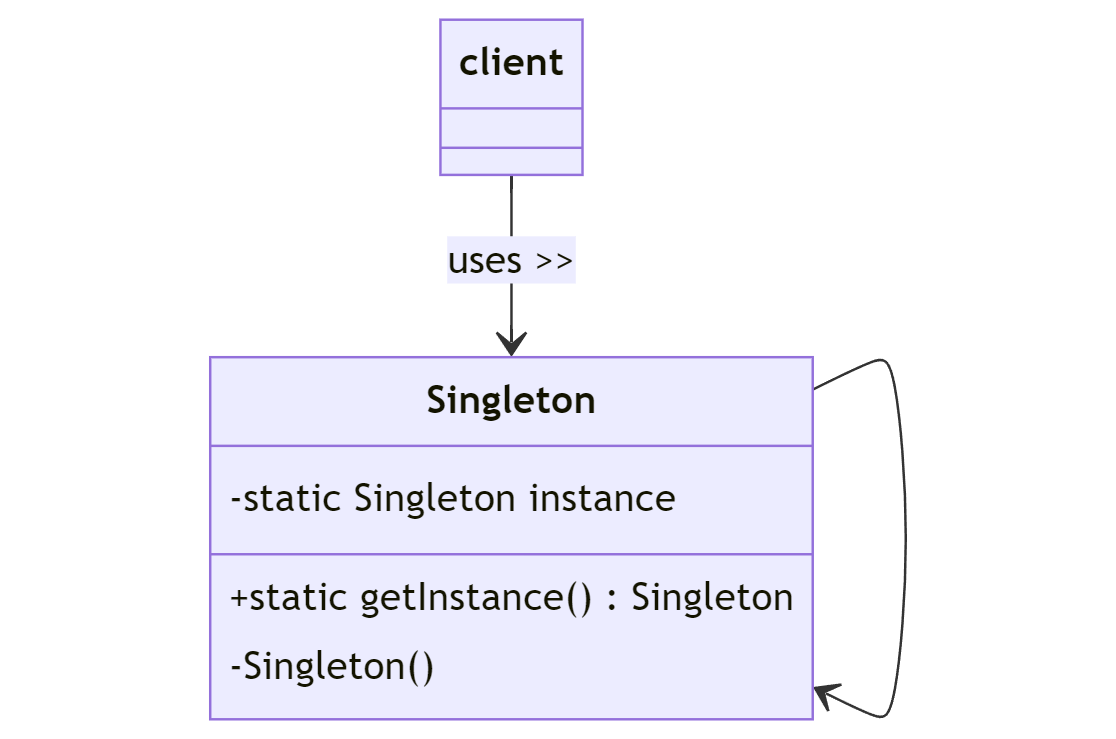
\includegraphics[scale=0.2]{classe_singleton.png}
        \label{fig:SingletonClassDiagram}
    \end{figure}
\hfill
    \begin{figure} [!ht]
        \centering
        \caption{Diagramme de séquence pour le Singleton}
        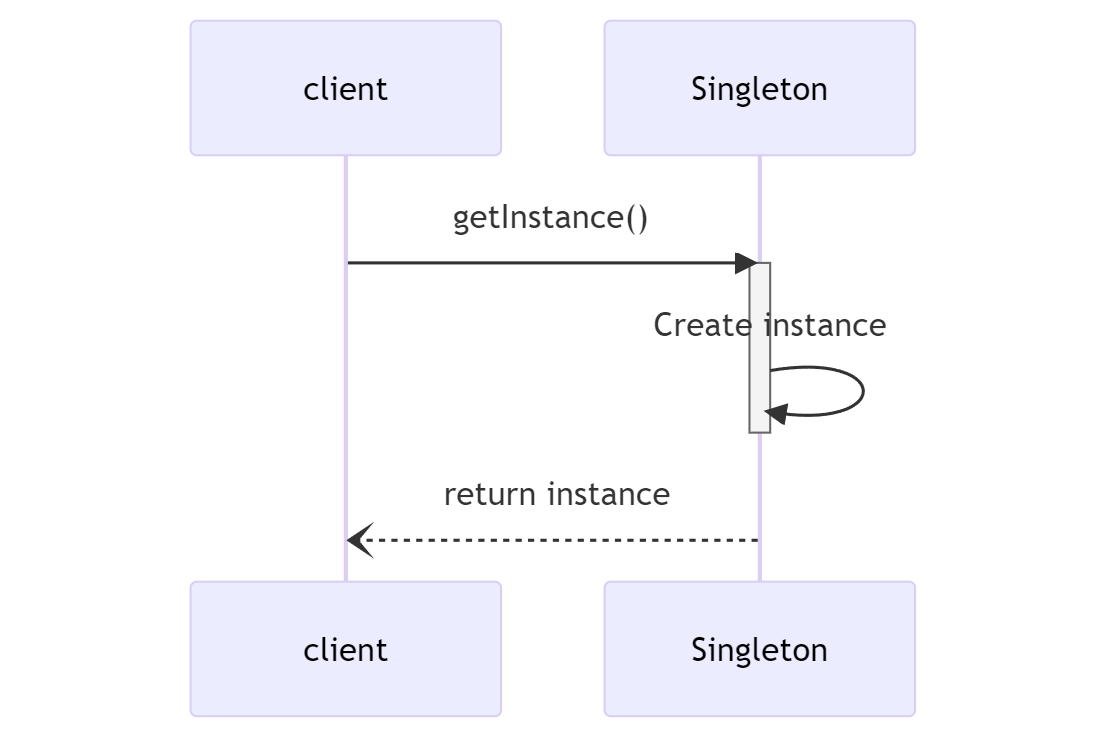
\includegraphics[scale=0.2]{sequence_singleton.png}
        \label{fig:SingletonSequenceDiagram}
    \end{figure}

    
\pagebreak
    \item \textbf{Factory} \\
    La Factory a été employée pour décentraliser la création d'éléments de l'interface utilisateur, facilitant la gestion et l'extension des menus ainsi que les shapes. Les classes Factory concrètes sont utilisées pour instancier les objets menu en fonction des besoins de l'utilisateur sans coupler le code à des implémentations spécifiques.

    \begin{figure} [!ht]
        \centering
        \caption{Diagramme de classe pour le Factory}
        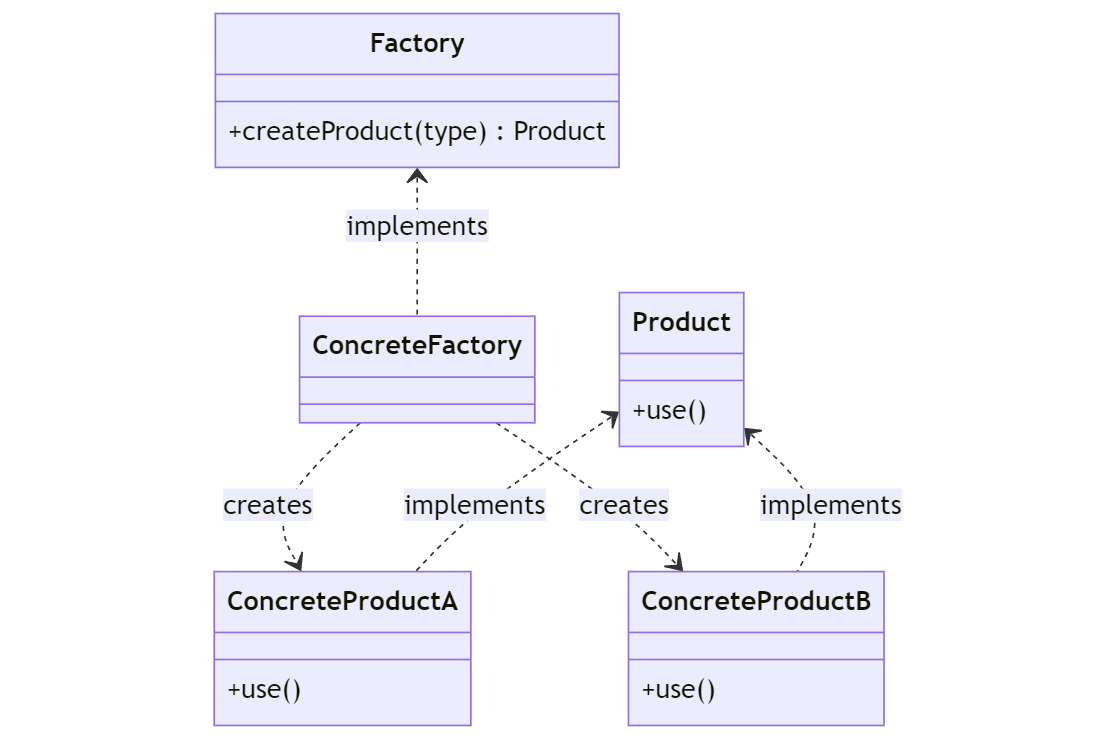
\includegraphics[scale=0.3]{classe_factory.png}
        \label{fig:FactoryClassDiagram}
    \end{figure}

    \begin{figure} [!ht]
        \centering
        \caption{Diagramme de séquence pour le Factory}
        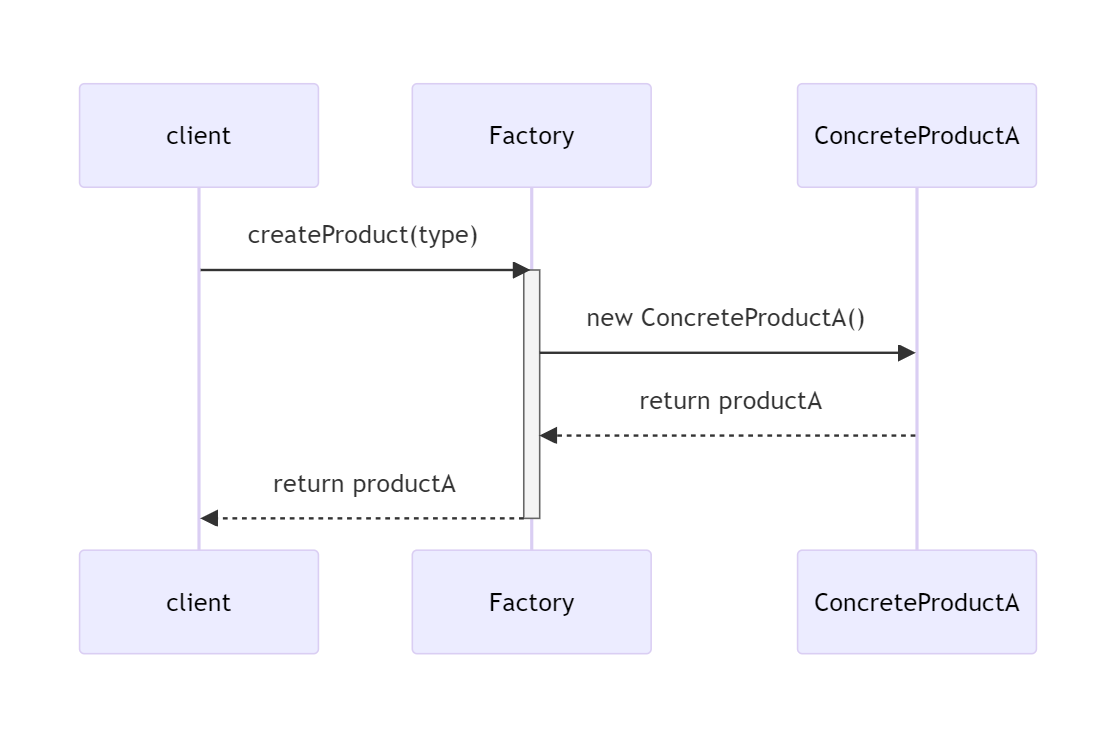
\includegraphics[scale=0.3]{sequence_factory.png}
        \label{fig:FactorySequenceDiagram}
    \end{figure}
\pagebreak
    \item \textbf{Composition} \\
    Le pattern Composition a été mis en place pour organiser les formes géométriques, permettant aux utilisateurs de manipuler des ensembles de formes comme s'ils étaient une entité unique. Cette structuration aide à gérer des modifications groupées et des interactions complexes entre objets composites.

    \begin{figure} [!ht]
        \centering
        \caption{Diagramme de classe pour le Composition}
        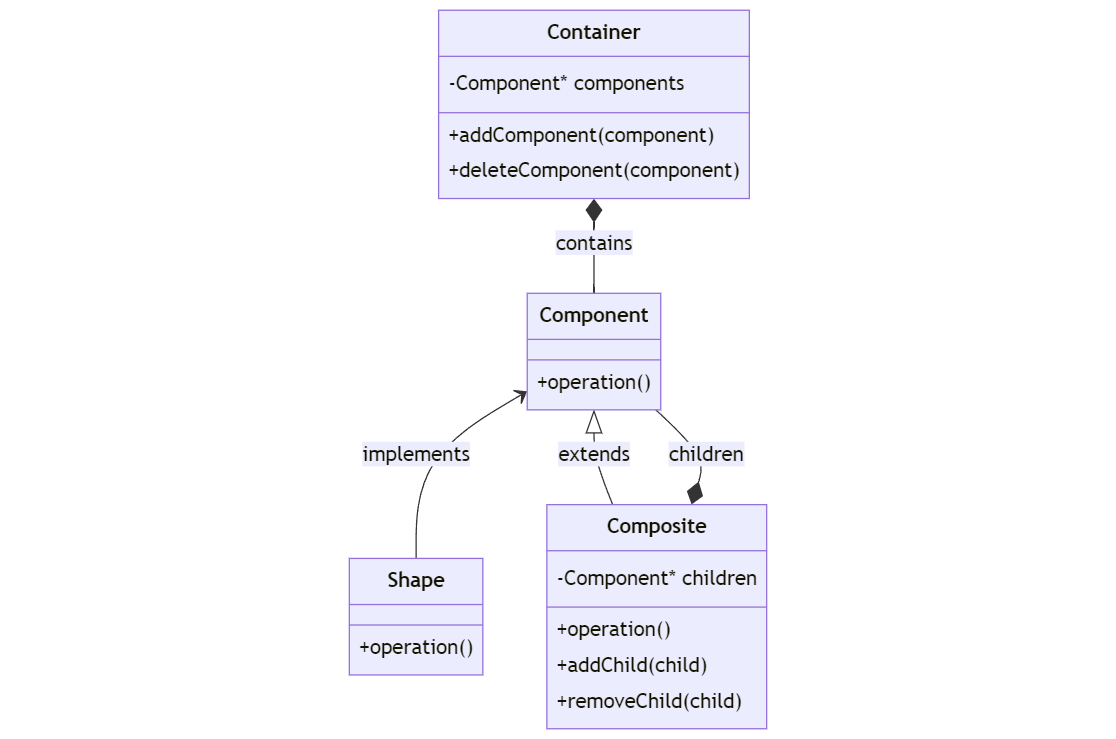
\includegraphics[scale=0.3]{classe_composition.png}
        \label{fig:CompositionClassDiagram}
    \end{figure}
    
    \begin{figure} [!ht]
        \centering
        \caption{Diagramme de séquence pour le Composition}
        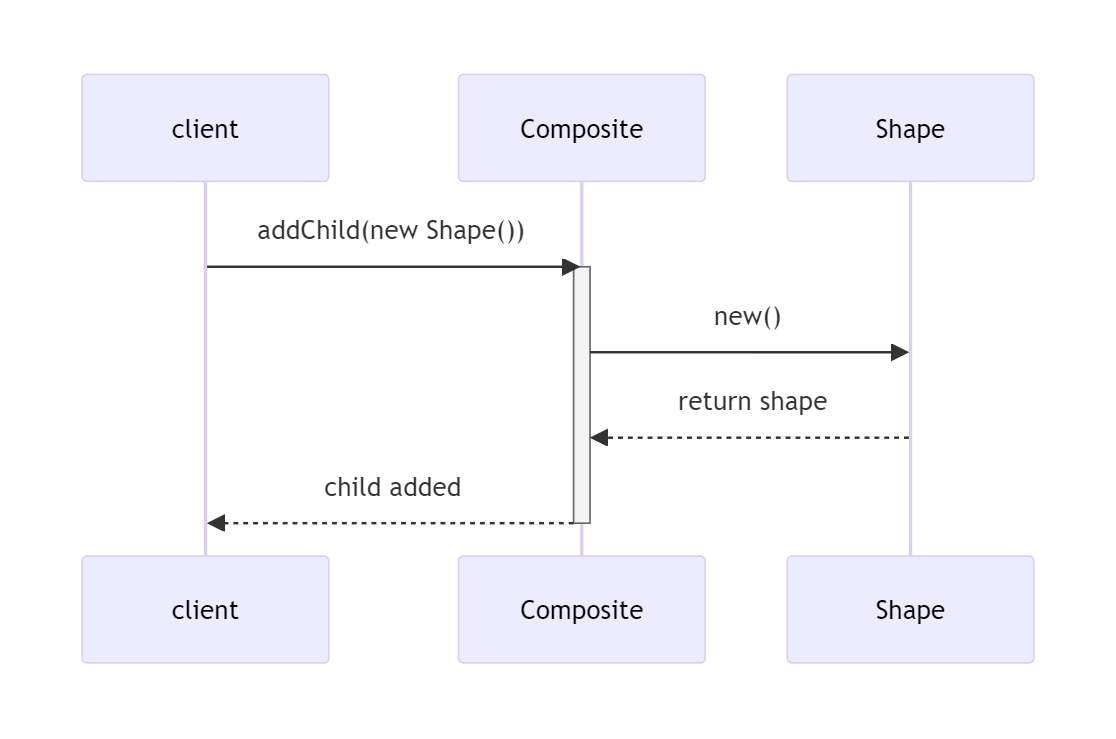
\includegraphics[scale=0.3]{sequence_composition.png}
        \label{fig:CompositionSequenceDiagram}
    \end{figure}
\pagebreak
    \item \textbf{Prototype} \\
    Abstract Factory a été utilisé pour fournir une interface pour la création de familles de formes sans spécifier leurs classes exactes. Cela permet l'extension de l'application avec de nouvelles formes sans modifier le code existant.
    
    \begin{figure} [!ht]
        \centering
        \caption{Diagramme de classe pour Prototype}
        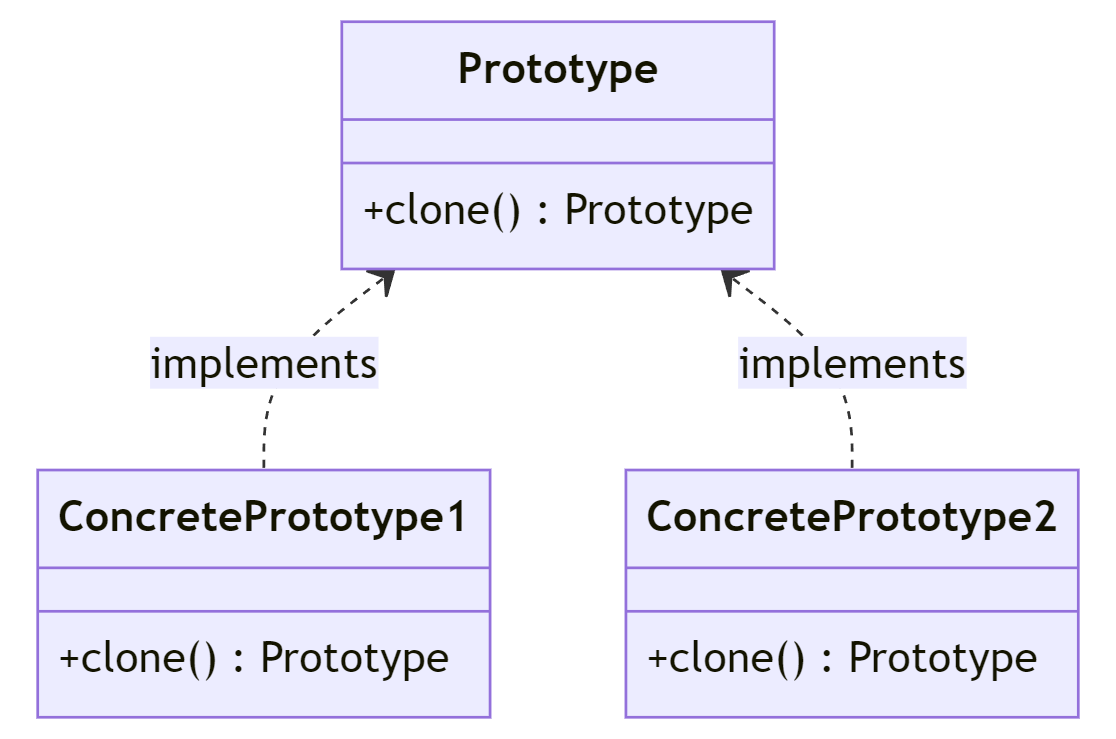
\includegraphics[scale=0.2]{classe_prototype.png}
        \label{fig:AbstractFactoryClassDiagram}
    \end{figure}

    \begin{figure} [!ht]
        \centering
        \caption{Diagramme de séquence pour Prototype}
        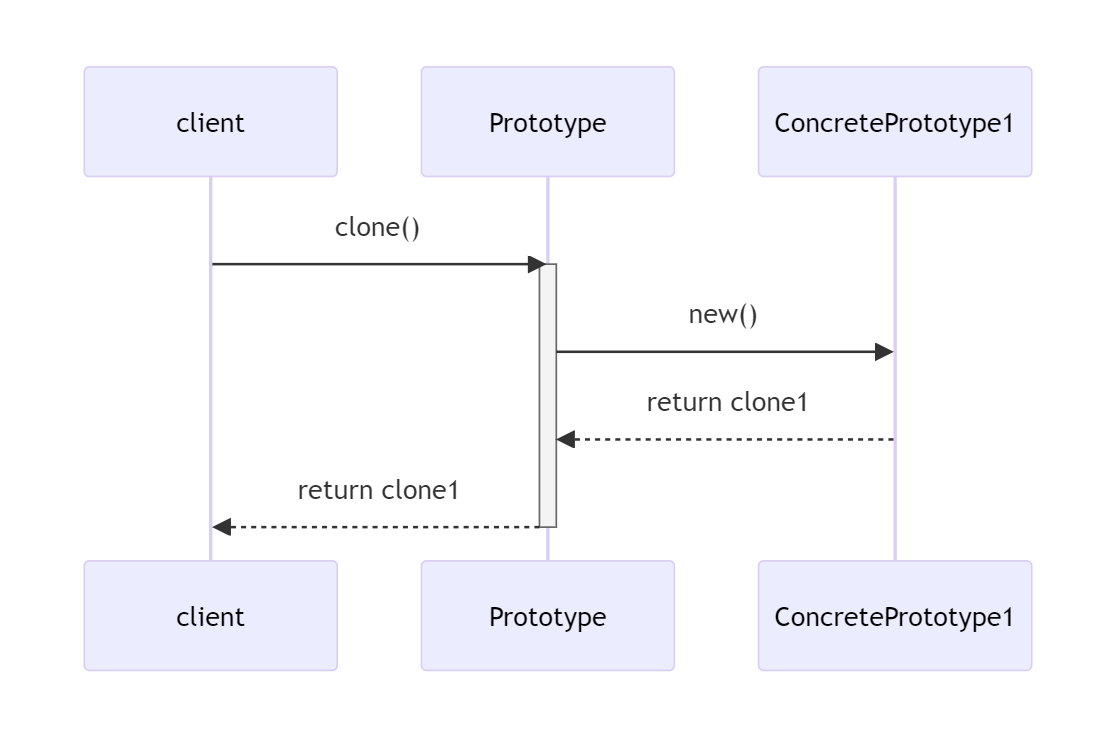
\includegraphics[scale=0.3]{sequence_prototype.png}
        \label{fig:AbstractFactorySequenceDiagram}
    \end{figure}
\pagebreak
    \item \textbf{Command} \\
    L'architecture Command a été intégrée pour encapsuler toutes les interaction des utilisateurs possibles en tant qu'objets de commande, pour une plus grande modularité dans le traitement des interactions utilisateur, rendant le code plus adaptable et plus facile à tester.

    \begin{figure} [!ht]
        \centering
        \caption{Diagramme de classe pour le Command}
        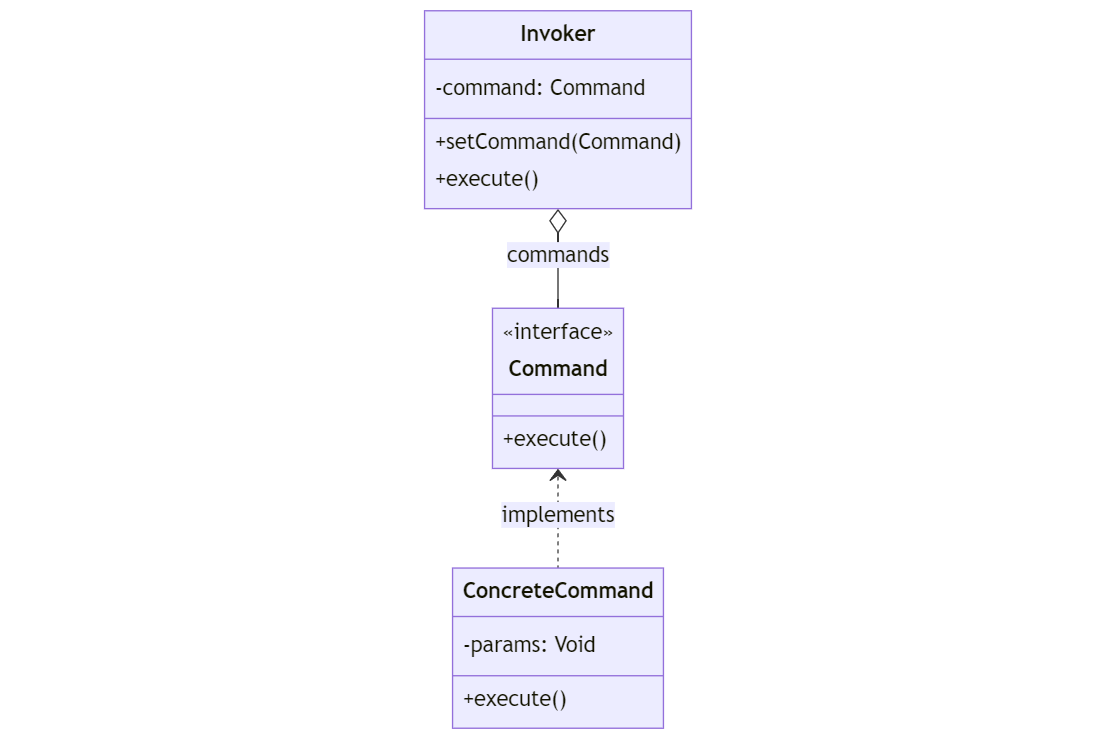
\includegraphics[scale=0.3]{classe_command.png}
        \label{fig:CommandClassDiagram}
    \end{figure}

    \begin{figure} [!ht]
        \centering
        \caption{Diagramme de séquence pour le Command}
        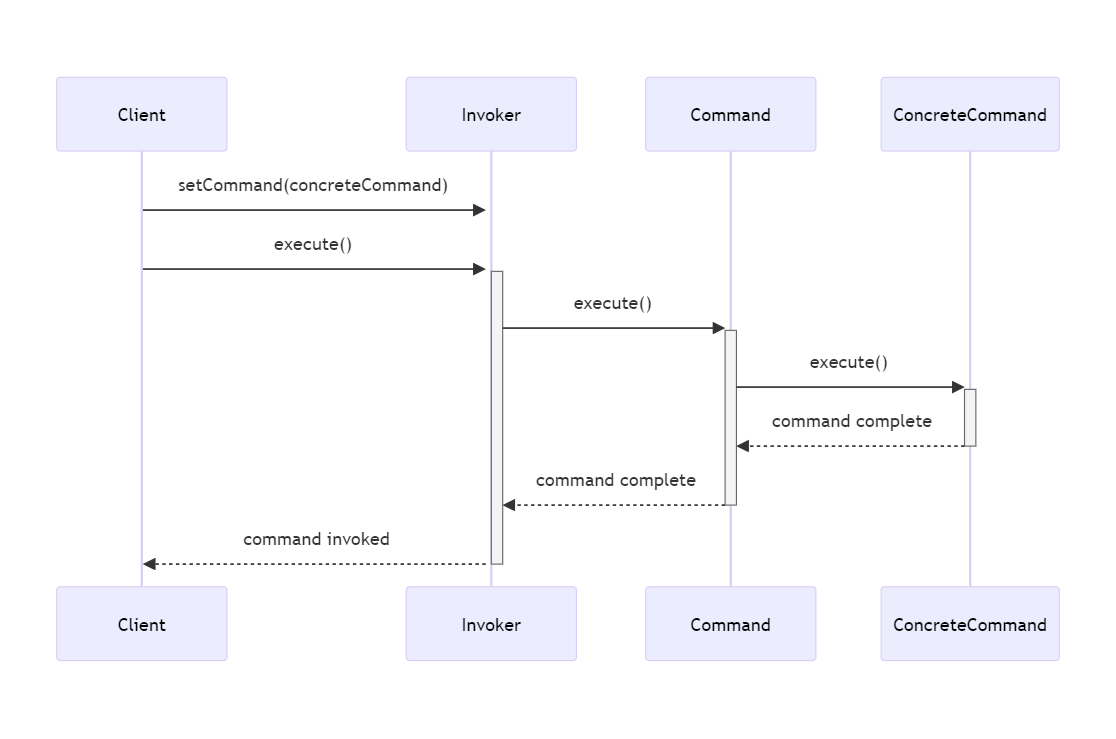
\includegraphics[scale=0.3]{sequence_command.png}
        \label{fig:CommandSequenceDiagram}
    \end{figure}
\pagebreak
    \item \textbf{Memento} \\
    Memento a été crucial pour l'implémentation des fonctionnalités d'undo/redo ainsi qu'aux système de backup, permettant aux utilisateurs de revenir à un état précédent sans perdre l'intégrité de l'état de l'application. Ce système stocke les états précédents de manière efficace, en veillant à ce que l'utilisateur puisse faire des modifications sans risque.

    \begin{figure} [!ht]
        \centering
        \caption{Diagramme de classe pour le Memento}
        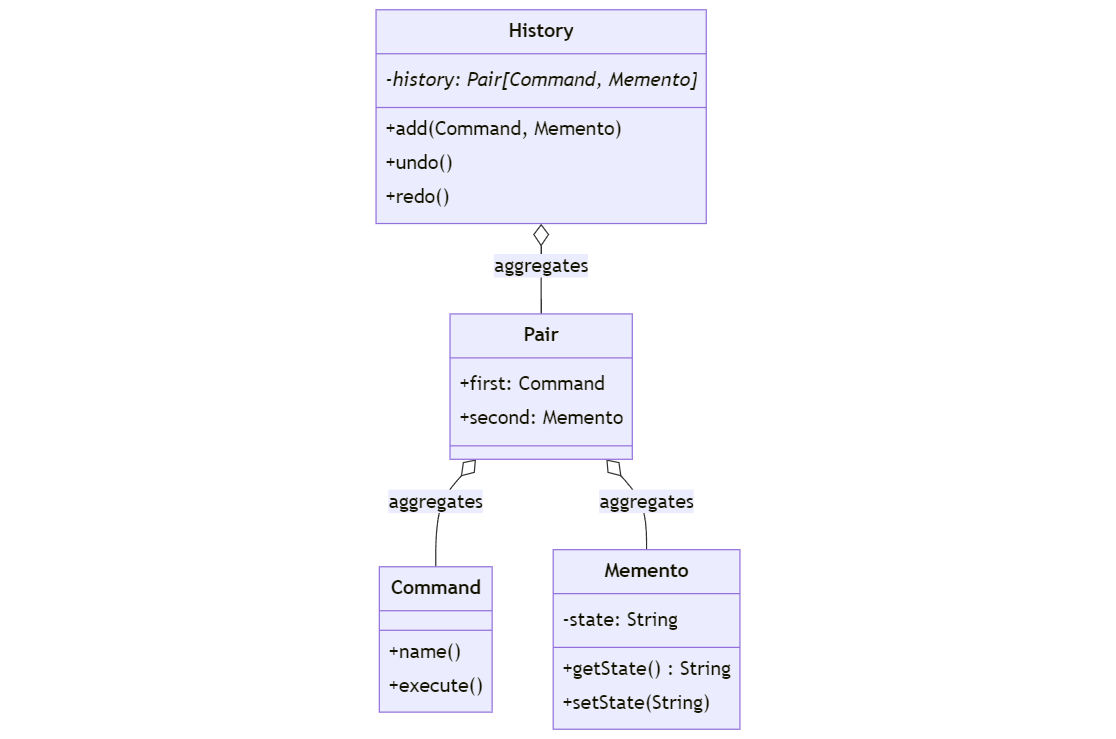
\includegraphics[scale=0.3]{classe_memento.png}
        \label{fig:MementoClassDiagram}
    \end{figure}

    \begin{figure} [!ht]
        \centering
        \caption{Diagramme de séquence pour le Memento}
        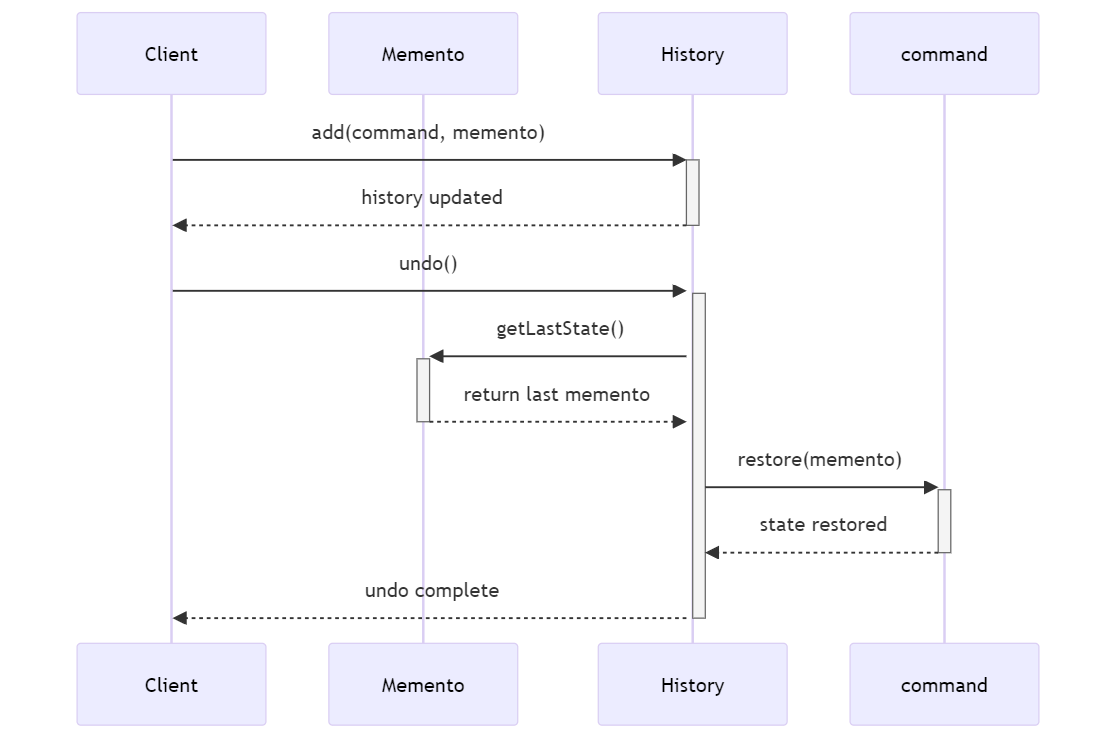
\includegraphics[scale=0.3]{sequence_memento.png}
        \label{fig:MementoSequenceDiagram}
    \end{figure}
\end{enumerate}

\pagebreak
\subsection{Tests et validation}
Tous les cas d'utilisation définis pour l'application ont été exécutés avec succès, confirmant ainsi que chaque fonctionnalité fonctionne correctement et répond aux exigences spécifiées.
\begin{enumerate}
    \item \textbf{Glissé-déposer depuis la toolbar}:
    \begin{enumerate}
        \item L'utilisateur clique sur un élément de la toolbar.
        \item Il effectue un glissé-déposer.
        \item Il relâche son clic :
        \begin{itemize}
            \item Au-dessus de la feuille blanche, une nouvelle instance de l'objet est ajoutée à la feuille de dessin.
            \item Dans une icône "Poubelle", l'élément est supprimé de la toolbar.
            \item Ailleurs, rien ne se passe.
        \end{itemize}
    \end{enumerate}
    \item \textbf{Groupage}:
    \begin{enumerate}
        \item L'utilisateur réalise une sélection potentiellement multiple d'objets.
        \item La sélection peut se faire soit via un rectangle de sélection sur le whiteboard, soit par control-clics successifs.
        \item Il sélectionne l'option "Group" d'un menu en clic-droit.
        \item Les objets deviennent enfants d'un groupe d'objets.
    \end{enumerate}
    \item \textbf{Dissociation d'un groupe}:
    \begin{enumerate}
        \item L'utilisateur sélectionne un groupe d'objets.
        \item Il sélectionne l'option "De-group" d'un menu en clic-droit.
        \item Les objets sont dégroupés, c'est-à-dire rajoutés au groupe parent. Ils ne doivent pas changer de position, etc.
    \end{enumerate}
    \item \textbf{Édition des propriétés des objets}:
    \begin{enumerate}
        \item L'utilisateur sélectionne un objet ou un groupe d'objets.
        \item Il réalise un clic droit et sélectionne "Edit" dans un menu déroulant.
        \item Une boîte de dialogue s'ouvre : elle contient les paramètres que l'on peut modifier.
        \item L'utilisateur change un ou plusieurs des paramètres.
        \item Il appuie sur :
        \begin{itemize}
            \item "Appliquer" : les modifications sont appliquées, et il peut continuer à changer des paramètres.
            \item "Ok" : les modifications sont appliquées et le dialogue se ferme.
            \item "Annuler" : toutes les modifications réalisées depuis l'ouverture du dialogue sont annulées.
        \end{itemize}
    \end{enumerate}
    \item \textbf{Glissé-déposé vers toolbar}:
    \begin{enumerate}
        \item L'utilisateur sélectionne un objet ou groupe d'objets.
        \item Il effectue un drag'n'drop.
        \item S'il relâche la souris sur la toolbar, un nouvel élément est ajouté dans la toolbar.
        \item S'il relâche la souris sur la poubelle, les objets sont supprimés.
    \end{enumerate}
\end{enumerate}
\pagebreak
\subsection{Difficultés rencontrées}

Le développement de l'application a été marqué par plusieurs défis techniques et conceptuels. Voici les principales difficultés rencontrées :

\begin{itemize}
    \item \textbf{Démarrage avec AWT} : L'utilisation de Java AWT pour la gestion des interfaces graphiques a présenté des défis dès le début du projet. Des incompréhensions sur l'utilisation de certains composants ont ralenti les premières phases de développement. La solution a été de consulter des ressources complémentaires et des forums en ligne, ainsi que de réaliser de petits prototypes pour tester les fonctionnalités avant leur intégration.

    \item \textbf{Gestion du redimensionnement} : La fonctionnalité de redimensionnement des formes géométriques a impliqué des calculs complexes pour maintenir les proportions et les alignements corrects. Les difficultés résidaient dans la coordination des dimensions en fonction des transformations et des contraintes d'affichage.

    \item \textbf{Copie des objets} : La mise en œuvre de la fonctionnalité de copie s'est heurtée à des problèmes liés à la copie partielle des objets via l'interface Cloneable de Java, qui ne permettait pas de copier en profondeur des structures d'objets complexes. Cela a conduit à des bugs liés aux pointeurs entre les objets clonés. Une méthode de copie profonde personnalisée a du être implémentée pour s'assurer que chaque composant de l'objet était correctement reproduit sans partager de références avec l'original.

    \item \textbf{Gestion du focus} : La coordination du focus entre le clavier et la souris s'est révélée complexe, particulièrement dans un environnement riche en éléments interactifs. Les problèmes concernaient la détermination de l'élément ayant le focus pour les entrées du clavier après des interactions avec la souris. Des ajustements dans la gestion des événements à été nécessaires pour garantir une manipulation intuitive et cohérente du focus.
\end{itemize}


\subsection{Ajout supplémentaires}

Pour améliorer l'efficacité et l'intuitivité de l'utilisation de l'application, plusieurs raccourcis clavier et fonctionnalités supplémentaires ont été ajoutés. Ces ajouts sont destinés à optimiser les flux de travail des utilisateurs et à accroître la rapidité des interactions avec l'application.

\begin{itemize}
    \item \textbf{CTRL+S (Sauvegarde)} : Implémenter un raccourci pour la sauvegarde rapide des projets en cours. Cela permettra aux utilisateurs de sécuriser régulièrement leur travail sans interrompre leur processus créatif.
    
    \item \textbf{CTRL+O (Ouverture)} : Un raccourci pour ouvrir rapidement un projet existant. Ce raccourci facilitera l'accès aux travaux précédents, rendant le processus de chargement des fichiers plus fluide et moins intrusif.
    
    \item \textbf{CTRL+Z (Annuler)} : Renforcer la fonctionnalité d'annulation pour permettre aux utilisateurs de revenir facilement sur leurs dernières actions. Ce raccourci est essentiel pour une exploration créative sans risque.
    
    \item \textbf{CTRL+Y (Refaire)} : Complémentaire à l'annulation, ce raccourci permettra de rétablir les actions précédemment annulées.
    
    \item \textbf{CTRL+G (Groupage)} : Un raccourci pour grouper rapidement plusieurs objets sélectionnés. Ce raccourci accélérera les modifications complexes en permettant aux utilisateurs de manipuler des groupes d'objets comme s'ils étaient une entité unique.
    
    \item \textbf{Suppression depuis la toolbar d'une shape} : Permettre aux utilisateurs de supprimer directement des formes de la toolbar via un mécanisme de suppression pour ne pas surchargé la toolbar inutilement. Cette fonctionnalité ajoutera une couche de personnalisation à l'interface utilisateur, permettant aux utilisateurs de mieux organiser et personnaliser leur espace de travail.
\end{itemize}


\subsection{Pistes d'amélioration}
En vue d'une amélioration à grande échelle de l'application, voici une liste exhaustive de certaines améliorations qui pourraient être possibles. Ces propositions visent à améliorer la performance, l'utilisabilité et l'efficacité de l'application, tout en tenant compte des défis technologiques actuels et futurs.

\begin{enumerate}
    \item \textbf{Déplacement simultané} : 
    Actuellement, le déplacement de plusieurs objets non groupés doit être effectué individuellement. L'intégration d'une fonctionnalité permettant le déplacement simultané de plusieurs éléments sélectionnés qui ne sont pas groupés améliorerait significativement l'expérience utilisateur.

    \item \textbf{Gestion de la mémoire cache} :
    L'implémentation d'une gestion de la mémoire cache pourrait considérablement améliorer la réactivité et l'efficacité de l'application, particulièrement pour les opérations qui nécessitent un accès rapide et répété à certaines données, comme le rendu des formes ou les fonctionnalités d'undo/redo. Cela pourrait également réduire la charge sur la mémoire principale et accélérer le traitement des données, en particulier pour les utilisateurs travaillant sur des projets complexes avec de nombreux éléments graphiques.

    \item \textbf{Ajout de thread} :
    L'intégration de threads pour gérer les calculs en parallèle pourrait significativement augmenter la vitesse et la réactivité de l'application lors de l'exécution de tâches multiples ou complexes. Cela serait particulièrement utile pour des opérations comme le recalcul de la géométrie des formes, le rendu en temps réel ou encore la gestion simultanée de multiples entrées utilisateur.

    \item \textbf{Rétrocompatibilité} : 
    Assurer la rétrocompatibilité des sauvegardes lors des mises à jour du logiciel pour éviter la perte de données. Il est important que les fichiers sauvegardés avec les versions antérieures restent utilisables avec les nouvelles versions du logiciel.
    
\end{enumerate}
\pagebreak
\section{Exécution}

\subsection{Exécution .exe}

\subsection{Commande d'exécution}

Il est possible d'exécuter l'application via le fichier .exe généré. en utilisant la commande suivante :


\begin{lstlisting}[language=bash,caption={Command execution .exe}]
cd ./executable
./FigmaV2.exe
\end{lstlisting}

\subsection{Exécution .jar}
\subsubsection{Prérequis}

- \textbf{JDK Requis :} JDK 21.\\ Assurez-vous que au moins le JDK 21 est installé sur votre machine. La version du JDK est disponible depuis le site officiel d'Oracle ou directement via ce lien : \url{https://download.oracle.com/java/21/latest/jdk-21_windows-x64_bin.exe}

\subsubsection{Commande d'exécution}

Pour exécuter l'application sous Windows, utilisez la commande suivante dans PowerShell. Assurez-vous que le chemin d'accès à votre JAR et à votre JDK est correct et que votre classe principale est correctement spécifiée :

\begin{lstlisting}[language=bash,caption={Command execution .jar}]
& "C:\Program Files\Java\jdk-21\bin\java.exe" -cp ".\FigmaV2-1.0-SNAPSHOT.jar" thibault.kuraima.Main
\end{lstlisting}

\pagebreak
\bibliographystyle{plainurl}
\bibliography{biblio}

\end{document}%